Ce chapitre comporte la théorie physique du mouvement d'un pendule qui vise à obtenir les équations du système. Les équations et schémas de
cette partie sont directement tirés ou inspirés du papier sur la modélisation et régulation d'un pendule inversé rédigé par Freddy Mudry \cite{FreddyMudry}.\\

Pour illustrer les propos, la figure \ref{fig:Illustration} est réutilisée et séparée en plusieurs partie pour observer les forces entre les
les pièces du montage. Ceci permet de faire les calculs de dynamique du système.

\begin{figure}[H]
    \centering
    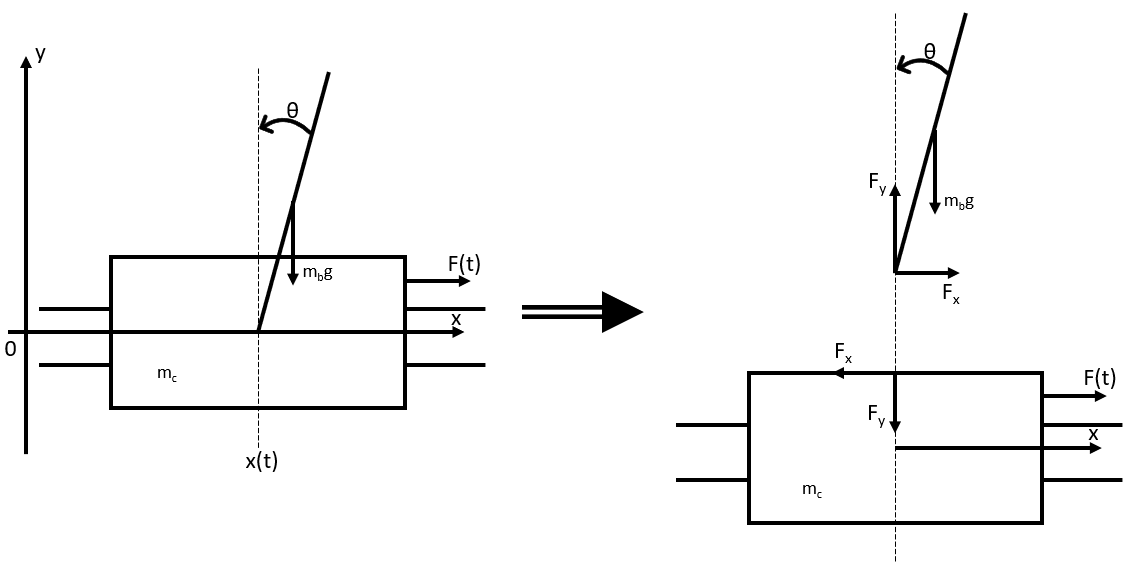
\includegraphics[width = 0.9\textwidth]{assets/figures/SchemaPhysiquePendule.svg}
    \caption{Illustration du pendule inversé demandé}
    \label{fig:Illustration2}
\end{figure}

La position linéaire est donc définie comme étant x et la position angulaire comme étant $\theta$. Les variable suivantes sont aussi définie.

\begin{itemize}
    \item Demi-longueur de la tige: $l$
    \item Masse du chariot: $m_c$
    \item Masse du pendule: $m_p$
    \item Inertie de rotation: $J$
    \item Force appliquée sur le chariot: $F$
\end{itemize}

Avec la masse totale $M = m_c + m_p$ et $J = m_b\frac{l^2}{3}$

\section{Équations du balancier}\label{sec:EqBal}
Les équations du balancier se font autour du centre de gravité de la tige qui est défini par ses coordonnées en x et y par les variables $x_G$
et $y_G$. Ces dernières sont l'application de la seconde loi de Newton sur l'axe x et l'axe y avec des forces et sur l'axe z avec des moments.

\begin{equation}\label{eq:SecondNewtX}
    m_b\ddot{x_G} = F_x
\end{equation}

\begin{equation}\label{eq:SecondNewtY}
    m_b\ddot{y_G} = F_y - m_bg
\end{equation}

\begin{equation}\label{eq:SecondNewtMom}
    J\ddot{\theta}(t) = lcos(\theta)F_x + lsin(\theta)F_y
\end{equation}

\section{Équations du chariot}\label{sec:EqChar}
Le chariot peut se déplacer uniquement le long de l'axe x ce qui signifie qu'il ne possède qu'une seule équation.

\begin{equation}\label{eq:SecondNewtX2}
    m_c\ddot{x} = F(t) - F_x
\end{equation}

\section{Équations de liaison}\label{sec:EqLiaison}
Le centre de gravité de la tige se calcule avec les équations suivantes.

\begin{equation*}
    x_G = x - lsin(\theta), \hspace{30pt} y_G = lcos(\theta)
\end{equation*}

La dérivée de ces équations donne les équations de la vitesse du centre de gravité selon les axes x et y.

\begin{equation*}
    \dot{x}_G = \dot{x} - l\dot{\theta}cos(\theta), \hspace{30pt} \dot{y}_G = -l\dot{\theta}sin(\theta)
\end{equation*}

Effectuer la dérivée encore une fois sur ces équations donne les équations de l'accélération du centre de gravité selon les axes x et y.

\begin{equation}\label{eq:SecondNewtXG}
    \ddot{x}_G = \ddot{x} - l\ddot{\theta}cos(\theta) + l\dot{\theta}^2sin(\theta)
\end{equation}

\begin{equation}\label{eq:SecondNewtYG}
    \ddot{y}_G = - l\ddot{\theta}sin(\theta) - l\dot{\theta}^2cos(\theta)
\end{equation}

\section{Calcul des accélérations}\label{sec:CalcAcc}
Avec ces 6 équations et leurs 6 inconnues on trouve les équations suivantes en commençant par mettre l'équation \ref{eq:SecondNewtXG}
dans l'équation \ref{eq:SecondNewtX}.

\begin{equation}\label{eq:ForceX}
    F_x = m_b\ddot{x} - m_bl\ddot{\theta}cos(\theta) + m_bl\dot{\theta}^2sin(\theta)
\end{equation}

Et en mettant l'équation \ref{eq:SecondNewtYG} dans l'équation \ref{eq:SecondNewtY}.

\begin{equation}\label{eq:ForceY}
    F_y = m_bg - m_bl\ddot{\theta}sin(\theta) + m_bl\dot{\theta}^2cos(\theta)
\end{equation}

Les deux équations \ref{eq:ForceX} et \ref{eq:ForceY} peuvent être mises dans l'équation \ref{eq:SecondNewtMom}.

\begin{equation*}
    J\ddot{\theta} = lcos(\theta)(m_b\ddot{x} - m_bl\ddot{\theta}cos(\theta) + m_bl\dot{\theta}^2sin(\theta)) + lsin(\theta)(m_bg - m_bl\ddot{\theta}sin(\theta) - m_bl\dot{\theta}^2cos(\theta))
\end{equation*}

Ce qui donne l'équation suivante après simplification.

\begin{equation}\label{eq:BalancierTheta}
    \ddot{\theta} = \frac{3}{4l}(\ddot{x}cos(\theta) + gsin(\theta))
\end{equation}

De plus, en mettant l'équation \ref{eq:ForceX} dans l'équation \ref{eq:SecondNewtMom}, l'équation suivante est obtenue.

\begin{equation}\label{eq:BalancierX}
    \ddot{x} = \frac{F(t) + m_bl}{M}(\ddot{\theta}(t)cos(\theta(t)) - \dot{\theta}(t)^2sin(\theta(t)))
\end{equation}

Les équations \ref{eq:BalancierTheta} et \ref{eq:BalancierX} sont les équations du balancier.